\documentclass[tikz,border=8pt]{standalone}
\usepackage{tikz}
\usepackage{pgfplots}
\usepackage{amsmath,amssymb}
\usepackage[T1]{fontenc}
\usepackage{lmodern}
\usepackage{xcolor}
\usetikzlibrary{arrows.meta,positioning,shapes.geometric,fit,calc,backgrounds,matrix}
\pgfplotsset{compat=1.18}
\definecolor{ink}{HTML}{18202A}
\definecolor{blue}{HTML}{2563EB}
\definecolor{bluefill}{HTML}{EAF1FF}
\definecolor{green}{HTML}{14804A}
\definecolor{greenfill}{HTML}{E8F6EE}
\definecolor{amber}{HTML}{B56A00}
\definecolor{amberfill}{HTML}{FFF3D6}
\definecolor{red}{HTML}{B42318}
\definecolor{redfill}{HTML}{FDECEC}
\definecolor{gray}{HTML}{667085}
\definecolor{light}{HTML}{F4F6F8}
\definecolor{linegray}{HTML}{C7CDD4}
\tikzset{
  box/.style={draw=ink, rounded corners=3pt, very thick, fill=white, align=center, inner sep=7pt, font=\sffamily\small},
  bluebox/.style={box, fill=bluefill, draw=blue},
  greenbox/.style={box, fill=greenfill, draw=green},
  amberbox/.style={box, fill=amberfill, draw=amber},
  redbox/.style={box, fill=redfill, draw=red},
  ghost/.style={draw=linegray, rounded corners=3pt, thick, fill=light, align=center, inner sep=7pt, font=\sffamily\small},
  label/.style={font=\sffamily\footnotesize, text=gray, align=center},
  title/.style={font=\sffamily\bfseries\large, text=ink, align=center},
  arrow/.style={-{Latex[length=3mm,width=2mm]}, very thick, draw=ink},
  bluearrow/.style={-{Latex[length=3mm,width=2mm]}, very thick, draw=blue},
  redarrow/.style={-{Latex[length=3mm,width=2mm]}, very thick, draw=red},
  greenarrow/.style={-{Latex[length=3mm,width=2mm]}, very thick, draw=green}
}

\begin{document}
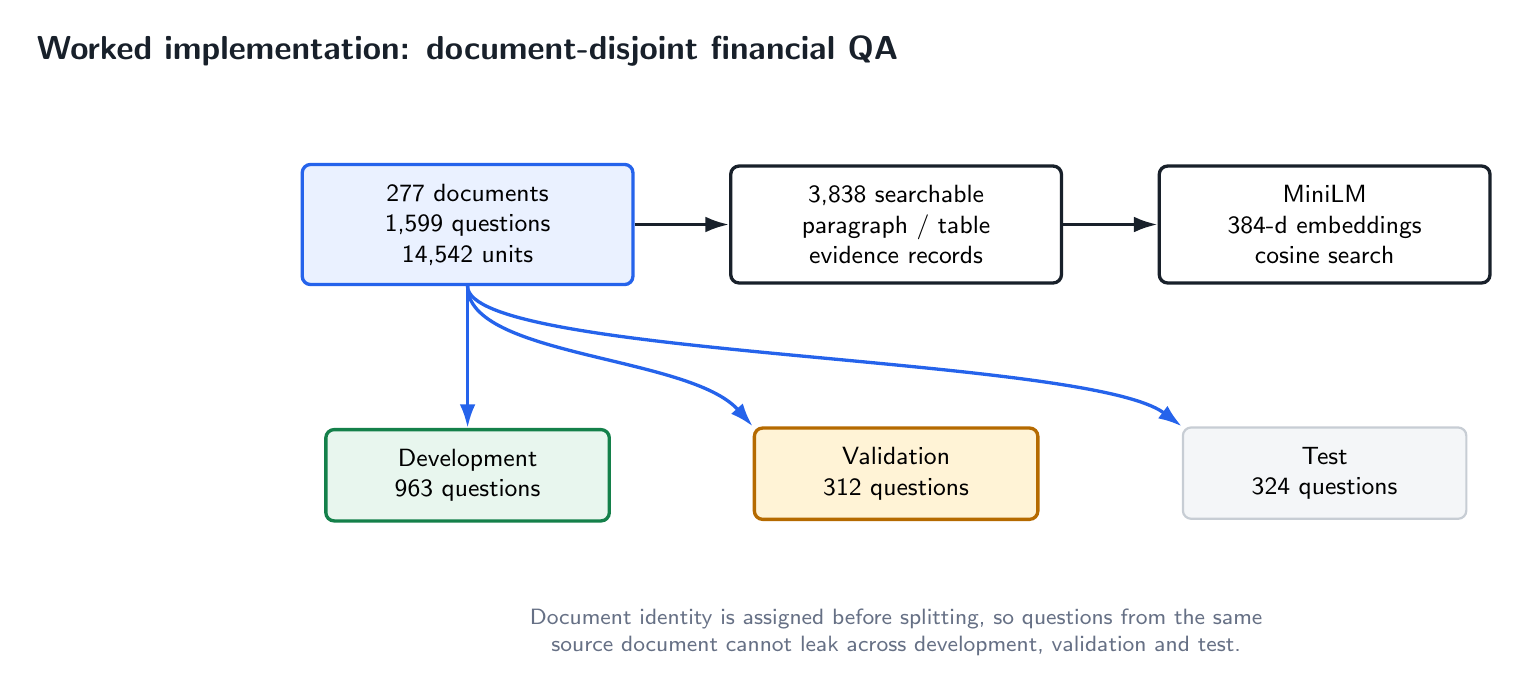
\begin{tikzpicture}[node distance=10mm and 12mm]
\node[title] (ttl) {Worked implementation: document-disjoint financial QA};
\node[bluebox, below=11mm of ttl, minimum width=42mm] (corp) {277 documents\\1,599 questions\\14,542 units};
\node[box, right=of corp, minimum width=42mm] (search) {3,838 searchable\\paragraph / table\\evidence records};
\node[box, right=of search, minimum width=42mm] (emb) {MiniLM\\384-d embeddings\\cosine search};
\draw[arrow] (corp)--(search); \draw[arrow] (search)--(emb);
\node[greenbox, below=18mm of corp, minimum width=36mm] (dev) {Development\\963 questions};
\node[amberbox, below=18mm of search, minimum width=36mm] (val) {Validation\\312 questions};
\node[ghost, below=18mm of emb, minimum width=36mm] (test) {Test\\324 questions};
\draw[bluearrow] (corp.south)--(dev.north); \draw[bluearrow] (corp.south) .. controls +(0,-9mm) and +(-8mm,9mm) .. (val.north west); \draw[bluearrow] (corp.south) .. controls +(0,-9mm) and +(-12mm,9mm) .. (test.north west);
\node[label, below=10mm of val, text width=130mm] {Document identity is assigned before splitting, so questions from the same source document cannot leak across development, validation and test.};
\end{tikzpicture}
\end{document}
